\title{An Autonomous Quadrotor Avoiding a Helicopter in Low-Altitude Flights}

\documentclass[journal,11pt,onecolumn,draftclsnofoot,]{IEEEtran}

\usepackage[noadjust]{cite}

% \usepackage{natbib}

\usepackage[left=1.25in,right=1.25in,top=1in,bottom=1in]{geometry}

\usepackage{amsmath}

\usepackage{color}

\usepackage[pdftex]{graphicx}

\usepackage{caption}
\usepackage{subcaption}
\intextsep = 0pt

\usepackage{array}

\usepackage{multicol}

\usepackage{url}

\usepackage[]{algorithm2e}

\usepackage{mwe}

\graphicspath{{./figure/}}

\ifCLASSOPTIONcompsoc
 \usepackage[caption=false,font=normalsize,labelfont=sf,textfont=sf]{subfig}
\else
 \usepackage[caption=false,font=footnotesize]{subfig}
\fi

\begin{document}
\title{An Autonomous Quadrotor Avoiding a Helicopter in Low-Altitude Flights}

\author{Zhilong Liu, Aislan G. Foina}

% Header
%\markboth{Header Here}
%{Shell \MakeLowercase{\textit{et al.}}: Bare Demo of IEEEtran.cls for Journals}

% show title
\maketitle
\pagenumbering{gobble}

\begin{abstract}
Drones are the first robots to arrive in smart cities, and collision avoidance with helicopters is among the first barriers to the widespread use of drones. In this paper, we develop control designs to analyze collision avoidance between quadrotors and helicopters. Communication radios, ADS-B for example, capable of broadcasting traffic information is regarded as a promising solution to the Sense and Avoid (SAA) problem for small Unmanned Aircraft Systems (sUAS), especially for high speed flights where long-range sensing is not possible. In this paper, a hybrid controller with ADS-B is introduced to enable a small quadrotor to perform optimal collision avoidance with a high-speed helicopter during autonomous navigation. First, a position controller and a safety controller are formulated independently. Then, they are combined together to form a hybrid automaton where transitions between the controllers are performed. Simulation shows the effectiveness of the hybrid controller.

\end{abstract}

% keywords
%\begin{IEEEkeywords}
%sliding mode, optimal control, collision avoidance, quadrotor.
%\end{IEEEkeywords}

% \IEEEpeerreviewmaketitle

\section{\textbf{Introduction}}

Recent advances in sensing and computing technology has made unmanned aerial vehicles/systems (UAV/UAS) low-cost but still increasingly capable of executing complex missions in challenging environments. They have gained popularity in a vast range of civilian applications, including search and rescue, disaster relief, and filming. Recently, the Federal Aviation Administration (FAA) has issued the Notice of Proposed Rulemaking (NPRM) on UAS certifications \cite{faa-nprm}, indicating that a large number of UAS will present in the National Airspace System (NAS) in the near future. Our research aims at small drones up to $25 kg$ traveling in class G airspace. Big value of this sort envisaged by Amazon Prime Air \cite{amazon_whitepaper_safe_access} happens only when the drone is able to fly itself tens of miles from the distribution center to people's homes autonomously. 

One prerequisite for such flights is collision avoidance. If thousands of drones were flying freely in urban areas without any safety control, they would become a huge danger to existing aircraft. A naive solution may require all drones to hover or land in the presence of manned aircraft. However, it will increase the operational cost of drones dramatically, making them no better than non-UAS competitive companies. This motivate us to develop a collision avoidance solution, to enable the UAS business without compromising today's manned aviation. This paper is a partial exploration of the drone collision avoidance problem in urban areas. Our main product is a hybrid controller that enables a UAS to perform collision avoidance with manned aircraft during autonomous navigation. 

To formulate the collision avoidance problem, we first identify the manned and unmanned aircraft of interest. Airspace management proposals from the FAA \cite{faa-nprm} and corporations such as Google \cite{google_airspace_system} and Amazon [\citen{amazon_whitepaper_safe_access}, \citen{amazon_whitepaper_airspace}] envisage drones flying below $150m$ in class G airspace, i.e., below all the aircraft carrying people. At this altitude, news, police, and medevac helicopters are the manned aircraft of interest \cite{google_airspace_system}. On the other hand, UAS flying in urban areas need vertical take-off, landing, hovering ability, and omni-directional maneuverability. This makes most urban UAS multirotors. Quadrotors are the simplest type of multirotors. Hence we focus on collision avoidance between quadrotors and helicopters. This is one of the first barriers to smart planes flying in smart cities \cite{google_airspace_system}.

In general, sense-and-avoid (SAA) technology could be divided into two categories, namely collaborative and non-collaborative. Non-collaborative SAA relies on remote sensing technologies, such as radars, laser range finders, and cameras, to detect obstacles. Aircraft with these sensors could detect a wide range of obstacles, including birds and buildings. However, for small UAS (sUAS) less than $25 kg$ \cite{faa-nprm}, we have limited payload capacity and limited detection range, typically less than $100m$ [\citen{art_sys_360},\citen{hokoyo_lidar}]. On the other hand, collaborative SAA relies on vehicle-to-vehicle (V2V) long-range communication, broadcasting and subscribing GPS-based traffic data of aircraft nearby. Google provides a discussion on collaborative SAA systems in \cite{google_airspace_system}. The transceiver candidates are Dedicated Short-Range Communications (DSRC) and Automatic Dependent Surveillance-Broadcast (ADS-B). The communication range goes from $900m$ (DSRC) \cite{msadaa2010comparative} to $24km$ (ADS-B) \cite{sagetech}. However, collaborative SAA also has several short-comings. First, the communication delay can be up to $1 s$ for ADS-B. Second, the position information is obtained from GPS, typically accurate to $5m$ near ground \cite{gps_accuracy}. In addition, obstacles outside the network are not detected. 

The collision avoidance problem of interest involves high-speed vehicles. Typical quadrotors and helicopters can travel at $30m/s$ and $70m/s$, respectively [\citen{quadrotor_common_speed}, \citen{helicopter_common_speed}]. In the worst-case head-on collision, assuming an avoidance reaction takes $5s$, then a range requirement of $500m$ is implied. This result completely excludes the possibility of non-collaborative SAA, whose maximum detection range is only $100 m$. In addition, the $500m$ range requirement also indicates its insensitivity to GPS position errors ($5m$, or $1\%$). Therefore, collaborative SAA is the only feasible choice. Recently, the FAA mandates that aircraft flying in the NAS must be equipped with ADS-B-out by 2020, which further stimulates the rapid growth of small-size ADS-B technology in the small UAS industry. Examples are XPG-TR from Sagetech \cite{sagetech} and ADS-B ONE from NextGen UAS Transponders \cite{ads-b-one}. In this paper, we assume that the vehicles of interest are equipped with ADS-B.

Given the collision detection mechanism, what remains is the navigation and collision avoidance algorithms, which constitute the contribution of this paper. The position controller is a set of concisely formulated sliding mode controllers augmented with dynamic surface control techniques. The safety controller generates optimal control actions when collisions are possible. We want to address the following scenario: A manned helicopter ambulance equipped with (ADS-B)-Out is flying at a low altitude to pick up a patient, when a quadrotor UAS with (ADS-B)-In is delivering packages autonomously. The quadrotor can receive real-time traffic information of the helicopter. If collision is possible, the quadrotor would avoid the manned helicopter. The avoidance maneuver is performed exclusively by the quadrotor UAS.

\section{\textbf{Literature Review}}

\subsection{Position Controller} \label{sec:pos_ctrl}

The quadrotor control literature can be divided into two classes. The first class focuses on attitude and altitude stabilization \cite{bouabdallah2004pid, li2011dynamic, madani2006backstepping_2, bouabdallah2005backstepping, bouadi2011adaptive}, while the second class controls the horizontal position as well \cite{lee2009feedback, xu2006sliding, taniguchi2014quadrotor}. Controlling the first class is straight forward because attitude and altitude are directly controlled by four independent control inputs. However, when horizontal position tracking is required, the problem becomes more difficult. The challenge is on resolving the underactuation issue, or using only four independent actuation inputs to handle all six degrees of freedom. Specifically, the tilting in roll and pitch are coupled with horizontal motions. To derive feasible horizontal control laws, the dynamic model is usually greatly simplified \cite{lee2009feedback, xu2006sliding} to avoid the explosion of terms when taking time derivatives.

In \cite{lee2009feedback}, Lee tried feedback linearization to fully control a quadrotor. The system model was reduced to include only thrust forces and gravity, and yet the derived control laws were quite lengthy. In addition, it augmented the state-space model with control inputs as additional states, yielding complicated dynamical input control laws. In \cite{taniguchi2014quadrotor}, another similar feedback linearization method with dynamic inputs was presented. The model in \cite{taniguchi2014quadrotor} was more complete, and the term explosion problem became huge! In summary, it is practically impossible to derive concise control laws from a full quadrotor model by directly applying nonlinear control methods.

In this paper, we resolve the term explosion problem by combining nonlinear control methods with dynamic surface control (DSC) techniques. Specifically, we augment the quadrotor model with two first-order filters from the DSC literature \cite{song2011dynamic}. With the DSC filters, we were able to access slightly lagged versions of the required time derivatives, and indirectly formulate concise control laws, to fully control a quadrotor, including horizontal positions.

\subsection{Avoidance Controller}

Collision avoidance designs entail assumptions on cooperation between aircraft. The most conservative strategy is to set up the problem as a non-cooperative pursuit evasion game \cite{lygeros1999controllers}, in which a helicopter is chasing a quadrotor. It would be ideal to permit the helicopter to do whatever it likes, but the difference in vehicle capability shows this to be infeasible. From \cite{helicopter_common_speed}, a typical maximum speed of commercial helicopters is $70m/s$. For a quadrotor, the maximum cruise speed is about $30m/s$ \cite{quadrotor_common_speed}. If a helicopter is deliberately chasing a quadrotor, the quadrotor would eventually be caught, regardless of its avoidance efforts. 

We focus instead on a semi-cooperative strategy, in which the responsibility for avoidance is placed on the quadrotor, and it gives way to the helicopter. This is also Google's current proposal \cite{google_airspace_system}. We capture this in two specific assumptions.

\begin{itemize}
	\item the quadrotor initiates the collision avoidance maneuvers;
	\item the helicopter maintains constant heading, altitude, and does not increase speed once the drone initiates collision avoidance.
\end{itemize}

The first attempt on addressing the collision avoidance problem in an optimal manner is presented in [\citen{schouwenaars2001mixed}, \citen{mellinger2012mixed}]. The avoidance problem is formulated as a path planning problem, in which the optimal path could be found by solving a mixed integer programming problem. The forbidden zone is set by rectangular constraints for simplicity. However, this is a centralized approach, which requires avoidance actions from both vehicles. In addition, solving MIQP becomes computationally expensive when the number of binary variables increases.

In \cite{hoffmann2008decentralized}, the collision avoidance problem between multiple quadrotors is solved by a decentralized optimal control approach. The optimal control is defined as the maximum acceleration with a constant optimal heading. Consequently, a real-time avoid set can be computed. The avoidance is activated only when collision becomes inevitable. However, the safety controller is derived from a simplified two-dimensional model. Once the controller is applied to a full 3D dynamic model, the optimality is not longer guaranteed because of rotational inertia and aerodynamic drag. Although the model difference is almost negligible in the low-acceleration ($\sim 1.5m/s^2$) low-speed ($\sim 2 m/s$) drone-drone avoidance scenario \cite{hoffmann2008decentralized}, it is no longer valid in high-acceleration ($\sim 10m/s^2$) high-speed ($\sim 100 m/s$) drone-helicopter scenario. 

In this paper, we modified the safety controller in \cite{hoffmann2008decentralized} to fit our drone-helicopter scenario. First, we only use the safety set from \cite{hoffmann2008decentralized} as an initial guess, and enlarge the safety set via an iterative algorithm to account for 3D dynamics. Second, this is a one-aircraft avoidance, where the only optimal control is the acceleration of the quadrotor, and the helicopter flies freely as if the quadrotor does not exist. 

\section{\textbf{Position Controller}}

\subsection{\textbf{Dynamic Model}} \label{sec:dynamic_model}

First, we need a quadrotor dynamic model. We adopt the same model introduced in \cite{bouadi2011adaptive}, with a different notation. Define a fixed north-east-down (NED) inertial world frame $\mathcal{W}$ and a non-inertial body frame $\mathcal{B}$ attached to the center of gravity of the quadrotor (Figure \ref{fig:frames}). The following is a list of variables used to describe the dynamics of a quadrotor.

\begin{itemize}
	\item $\boldsymbol{X}=[X\; Y\; Z]^T$: quadrotor position in $\mathcal{W}$;
	%		\item $\boldsymbol{x}=[x\; y\; z]^T$: quadrotor position in $\mathcal{B}$;
	\item $\boldsymbol{V}=[V_X\; V_Y\; V_Z]^T$: quadrotor velocity in $\mathcal{W}$;
	\item $\boldsymbol{\Theta}=[\phi\; \theta\; \psi]^T$: Euler angles roll, pitch, and yaw in $\mathcal{B}$, respectively;
	\item $\boldsymbol{\omega}=[\omega _x\; \omega _y\; \omega _z]^T$: quadrotor angular velocity in $\mathcal{B}$;
	\item $m$: quadrotor mass;
	\item $\boldsymbol{I}=diag(I_x,I_y,I_z)$: mass moment of inertia in $\mathcal{B}$;
	\item $\omega _{r_i}$: motor speeds, $i=1,2,3,4$;
	\item $\Omega=-\omega _{r_1}+\omega _{r_2}-\omega _{r_3}+\omega _{r_4}$: sum of motor speeds;
	\item $k_f, k_m$: motor thrust and torque coefficients, respectively;
	\item $c_t, c_r$: translational and rotational friction coefficients, respectively;
	\item $l$: moment arm from the origin of $\mathcal{B}$ to each motor.
	\item $\boldsymbol{g}$: gravitational acceleration, $[0 \; 0\; g]^T$  in NED frame with $g=9.81m/s^2$.
\end{itemize}

Assume that the motor forces are proportional to $\omega _{r_i}^2$, and the control inputs $\boldsymbol{U}$ satisfy (\ref{eq:controls}) with input constraints. Physically, the control inputs $U_1, U_2l, U_3l, U_4$ represent the total thrust and the total motor torques along the roll, pitch, and yaw axes, respectively. These are the control inputs for altitude and Euler angles. The constraints in (\ref{eq:controls}) represent the physical capacity of the motors.

Other forces are gravity $mg$, translation drag $c_t \boldsymbol{V}$, rotational drag $c_r \boldsymbol{\omega}^2$, and Coriolis forces from quadrotor body rotation and motor rotations. Define $R_{\mathcal{B}\rightarrow \mathcal{W}}$ to be the rotation matrix from $\mathcal{B}$ to $\mathcal{W}$, and $R_v$ to be a linear transformation from $\boldsymbol{\dot{\Theta}}$ to $\boldsymbol{\omega}$. The state-space equations could be written compactly as (\ref{eq:state_space_compact}). We only gives a brief summary of the model to introduce enough notations for controller conversions. For details, refer to \cite{bouadi2011adaptive}.

\begin{figure}
	\centering
	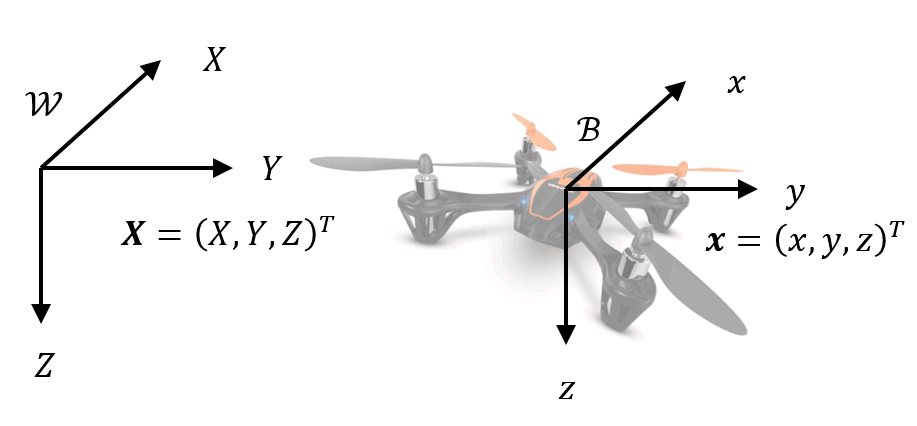
\includegraphics[width=0.5\columnwidth]{frames_quadrotor}
	\caption{The reference frames of a quadrotor.}
	\label{fig:frames}

\end{figure}

\begin{equation}
\label{eq:controls}
\begin{split}
\begin{matrix}
\begin{matrix}
\boldsymbol{U}=
\begin{bmatrix}
U_1\\ U_2\\ U_3\\ U_4
\end{bmatrix}
=
\begin{bmatrix}
k_f & k_f & k_f & k_f\\ 
0 & k_f & 0 & -k_f\\ 
k_f & 0 & -k_f & 0\\ 
k_m & -k_m & k_m & -k_m
\end{bmatrix}
\begin{bmatrix}
\omega _{r_1}^2\\ 
\omega _{r_2}^2\\ 
\omega _{r_3}^2\\ 
\omega _{r_4}^2
\end{bmatrix}\\
\end{matrix}
& \;\;\;\;
\begin{matrix}
0 &< U_1 \le 4 k_f \omega_{r,max}^2 \\
-k_f \omega_{r,max}^2 &\le U_2 \le k_f \omega_{r,max}^2 \\
-k_f \omega_{r,max}^2 &\le U_3 \le k_f \omega_{r,max}^2 \\
-2 k_m \omega_{r,max}^2 &\le U_4 \le 2 k_m \omega_{r,max}^2 \\
\end{matrix}
\end{matrix}
\end{split}
\end{equation}

%\begingroup\makeatletter\def\f@size{11}\check@mathfonts
\begin{equation}
\label{eq:state_space_compact}
\begin{split}
\boldsymbol{\dot{X}}&=\boldsymbol{V} \\
\boldsymbol{\dot{\Theta}}&=R_v^{-1}\boldsymbol{\omega} \\
\boldsymbol{\dot{V}}&=\boldsymbol{g}+\frac{1}{m}\left(-c_t\boldsymbol{V}+R_{\mathcal{B}\rightarrow \mathcal{W}}
\begin{bmatrix}
0\\ 0\\ U_1
\end{bmatrix}
\right) \\
\boldsymbol{\dot{\omega}}&=I^{-1} \left(\boldsymbol{\omega}\times \left(I\boldsymbol{\omega}\right)-\boldsymbol{\omega} \times \left(I_r 
\begin{bmatrix}
0\\ 0\\ \Omega
\end{bmatrix}
\right)-c_r \boldsymbol{\omega}^2+ 
\begin{bmatrix}
U_2l \\ U_3l \\ U_4
\end{bmatrix}
\right)
\end{split}
\end{equation}
%\endgroup



\subsection{\textbf{Sliding Mode Controllers with DSC Filters}} \label{sliding_controller}

Given the quadrotor model in Section \ref{sec:dynamic_model}, we can follow the standard procedure of designing sliding mode controllers, and formulate four independent control laws governing the altitude and attitudes (Euler angles) \cite{bouadi2011adaptive}, listed below in equation (\ref{eq:U1_4}) and (\ref{eq:U2_3}).

%\begingroup\makeatletter\def\f@size{9}\check@mathfonts
\begin{equation}
\label{eq:U1_4}
\begin{split}
U_1 &=  \frac{m}{c\phi c\theta} \left[ \left( -g+\frac{c_t}{m}V_Z + \ddot{Z}_d \right) - \lambda_Z \dot{e}_Z - \eta_Z sgn S_Z \right] \\
U_4 &=  I_z \left[ \left( -\frac{I_x-I_y}{I_z} \omega_x \omega_y + \frac{c_r}{I_z} \omega_z^2 + \ddot{\psi}_d \right) - \lambda_\psi \dot{e}_\psi\; - \eta_\psi sgn S_\psi \right] \\
\end{split}
\end{equation}
%\endgroup

%\begingroup\makeatletter\def\f@size{8}\check@mathfonts
\begin{equation}
\label{eq:U2_3}
\begin{split}
U_3 &= \frac{I_y}{l}\left[ \left( -\frac{I_z-I_x}{I_y} \omega_x \omega_z + \frac{c_r}{I_y} \omega_y^2 + \frac{I_r}{I_y} \Omega \omega_x \right)\; - \lambda_\theta \dot{e}_\theta \; - \eta_\theta sgn S_\theta \right] \\
U_2 &= \frac{I_x}{l}\left[ \left( -\frac{I_y-I_z}{I_x} \omega_y \omega_z + \frac{c_r}{I_x} \omega_x^2 + \frac{I_r}{I_x} \Omega \omega_y \right)\; - \lambda_\phi \dot{e}_\phi \; - \eta_\phi sgn S_\phi \right] \\
\end{split}
\end{equation}
%\endgroup

with tracking errors and sliding surfaces defined as in equation (\ref{eq:error_surfaces}), and $\lambda's$ and $\eta's$ as tuning parameters.

\begin{equation}
\label{eq:error_surfaces}
\begin{split}
\begin{matrix}
e_X \buildrel\triangle\over = X-X_d  & e_\theta \buildrel\triangle\over = \theta - \theta_d & S_X \buildrel\triangle\over = \dot{e}_X + \lambda_X e_X & S_\theta \buildrel\triangle\over = \dot{\theta} + \lambda_\theta e_\theta \\
e_Y \buildrel\triangle\over = Y-Y_d & e_\phi \buildrel\triangle\over = \phi - \phi_d  & S_Y \buildrel\triangle\over = \dot{e}_Y + \lambda_Y e_Y & S_\phi \buildrel\triangle\over = \dot{\phi} + \lambda_\phi e_\phi \\
e_Z \buildrel\triangle\over = Z-Z_d & e_\psi \buildrel\triangle\over = \psi-\psi_d & S_Z \buildrel\triangle\over = \dot{e}_Z + \lambda_Z e_Z & S_\psi \buildrel\triangle\over = \dot{e}_\psi + \lambda_\psi e_\psi \\
\end{matrix}
\end{split}
\end{equation}

Now, we can derive the horizontal control laws by augmenting our system with DSC filters. The overall horizontal motion control architecture is shown in Figure \ref{fig:horiz_ctrls}. It is a 3-step process. In the following, we show the design process in details.

\begin{figure}[thpb]
	\centering
	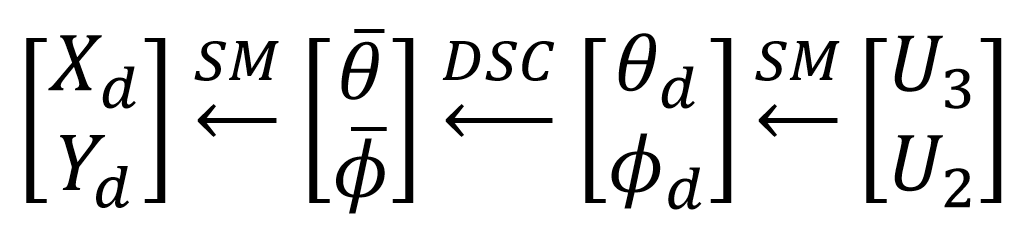
\includegraphics[width=2.5in]{horiz_ctrl}
	\caption{The horizontal motion control architecture.}
	\label{fig:horiz_ctrls}
\end{figure}

\subsubsection{derive synthetic inputs $\bar{\theta}$ and $\bar{\phi}$ via sliding mode (SM)}
First, take the time derivative of the sliding surfaces $S_X$ and $S_Y$ in (\ref{eq:error_surfaces}) and set them equal to the robustness terms with parameters $\eta_X$ and $\eta_Y$, respectively.
%\begin{equation}
%\label{eq:deriv_SS_XY}
%\begin{split}
%\dot{S}_X &= (\dot{V}_X - \ddot{X}_d) + \lambda_X \dot{e}_X \buildrel\triangle\over =-\eta_X sgn S_X \\
%\dot{S}_Y &= (\dot{V}_Y - \ddot{Y}_d) + \lambda_Y \dot{e}_Y \buildrel\triangle\over =-\eta_Y sgn S_Y  \\
%\end{split}
%\end{equation}
Then, substitute $\dot{V}_X$ and $\dot{V}_Y$ from (\ref{eq:state_space_compact}) and simplify with small angle approximations: $c\phi s\theta \approx \theta$ and $s\phi \approx \phi$, we have two new sliding mode control laws given by (\ref{eq:rp_synthetic_ctrls}).

\begin{equation}
\label{eq:rp_synthetic_ctrls}
\begin{split}
\begin{bmatrix}
\bar{\theta}\\ 
\bar{\phi}
\end{bmatrix}
= R(\psi) 
\begin{bmatrix}
\frac{m}{U_1} \left( \left( \frac{c_t}{m}V_X +\ddot{X}_d \right) - \lambda_X \dot{e}_X - \eta_X sgn S_X \right)\\
\frac{m}{U_1} \left( \left( \frac{c_t}{m}V_Y + \ddot{Y}_d \right) - \lambda_Y \dot{e}_Y - \eta_Y sgn S_Y \right)
\end{bmatrix}
\end{split}
\end{equation}

with rotation matrix

\begin{equation*}
\label{eq:R_yaw}
\begin{split}
R(\psi)  \buildrel\triangle\over =
\begin{bmatrix}
c\psi & s\psi \\ 
s\psi & -c\psi
\end{bmatrix}
\end{split}
\end{equation*}



Note that the roll $\bar{\theta}$ and $\bar{\phi}$ on the left-hand side of equation (\ref{eq:rp_synthetic_ctrls}) represent the synthetic controls for the desired horizontal motions. We distinguish them from the actual pitch $\theta$ and roll $\phi$.


\subsubsection{augment system with DSC filters}
To proceed, we need to somehow use equation (\ref{eq:rp_synthetic_ctrls}) in the time derivative of $S_\theta$ and $S_\phi$, so that the controls $U_3$ and $U_2$ can appear. However, as was mentioned in Section \ref{sec:pos_ctrl}, it requires taking time derivatives of (\ref{eq:rp_synthetic_ctrls}), which leads to explosion of terms. To avoid that, we instead augment the dynamic system (\ref{eq:state_space_compact}) with two first-order DSC filters shown in (\ref{eq:dsc_filters}), to indirectly converge the desired pitch $\theta_d$ and roll $\phi_d$ to the synthetic controls $\bar{\theta}$ and $\bar{\phi}$, respectively \cite{song2011dynamic}. The time constants $\tau_\theta$ and $\tau_\phi$ determine the convergence rates. The initial conditions are set to zeros in both filters. 

\begin{equation}
\label{eq:dsc_filters}
\begin{split}
\begin{matrix}
\tau _\theta \dot{\theta}_d+\theta_d = \bar{\theta}, & \theta_d(0) = 0 \\
\tau _\phi \dot{\phi}_d+\phi_d = \bar{\phi}, &             \phi_d(0) = 0\\
\end{matrix}
\end{split}
\end{equation}

The DSC filters (\ref{eq:dsc_filters}) allows us to compute $\dot{\theta}_d$ and $\dot{\phi}_d$ required in $\dot{S}_\theta$ and $\dot{S}_\phi$, without taking time derivatives of $\bar{\theta}$ and roll $\bar{\phi}$. Therefore, no simplifications in the dynamics are needed to accommodate the explosion of terms. A semi-global stability proof via Lyapunov analysis is lengthy because it involves the error dynamics  $(\dot{\theta}_d - \dot{\bar{\theta}})$ and $(\dot{\phi}_d - \dot{\bar{\phi}})$, which again involve explosion of terms. A standard proof is provided in \cite{song2011dynamic}. Here, we simply adopt the results.

\subsubsection{derive control inputs $U_3$ and $U_2$ via sliding mode (SM)}
Now we can take the time derivatives of $S_\theta$ and $S_\phi$, and set them equal to their robustness terms with parameters $\eta_\theta$ and $\eta_\phi$, respectively, with $\ddot{\theta} \approx \dot{\omega}_y$ and $\ddot{\phi} \approx \dot{\omega}_x$.

\begin{equation}
\label{eq:deriv_SS_rp}
\begin{split}
\dot{S}_\theta &\approx \dot{\omega}_y + \lambda_\theta ( \dot{\theta} - \dot{\theta}_d ) \buildrel\triangle\over =-\eta_\theta sgn S_\theta \\
\dot{S}_\phi &\approx \dot{\omega}_x + \lambda_\phi ( \dot{\phi} - \dot{\phi}_d ) \buildrel\triangle\over =-\eta_\phi sgn S_\phi \\
\end{split}
\end{equation}

In equation (\ref{eq:deriv_SS_rp}), $\dot{\omega}_y$ and $\dot{\omega}_x$ include the control inputs $U_3$ and $U_2$. They ($\dot{\omega}_y$ and $\dot{\omega}_x$), as well as $\dot{\theta}$ and $\dot{\phi}$, are given by (\ref{eq:state_space_compact}), and $\dot{\theta}_d$ and $\dot{\phi}_d$ are given by re-expressing the DSC filters as (\ref{eq:rp_des_deriv}).

\begin{equation}
\label{eq:rp_des_deriv}
\begin{split}
\dot{\theta}_d &= \frac{1}{\tau_\theta} \left( \bar{\theta} - \theta_d \right)\\
\dot{\phi}_d   &= \frac{1}{\tau_\phi} \left( \bar{\phi} - \phi_d \right)\\
\end{split}
\end{equation}

In equation (\ref{eq:rp_des_deriv}), $\bar{\theta}$ and $\bar{\phi}$ are given by (\ref{eq:rp_synthetic_ctrls}), and $\theta_d$ and $\phi_d$ are given by the DSC filter updates in (\ref{eq:dsc_filters}). Then, the horizontal control laws are given by (\ref{eq:U2_3}).

Lastly, the signum function ($sgn(\cdot)$) should be replaced by a smoothed function to avoid chattering. In this paper, we use a function with logistic and linear smoothing (\ref{eq:sgn_smoothed}).

\begin{equation}
\label{eq:sgn_smoothed}
\begin{split}
\eta sgn(S) &\leftarrow \left[ \eta_1\left( \frac{2}{1+e^{-cS}}-1 \right) + \eta_2 S \right] \\
\end{split}
\end{equation}

Throughout the derivation, we did not make any simplification to the full dynamic model (\ref{eq:state_space_compact}) other than small angle approximations. The innovation lies in the adoption of DSC filters.

\section{\textbf{Safety Controller}}

With the position controller, the quadrotor is capable of autonomous navigation to any given destinations. However, it is still prone to collision avoidance. In this section, the safety controller in \cite{hoffmann2008decentralized} is modified to accommodate the drone-helicopter avoidance scenario.

\subsection{Horizontal Safety Controller from Kinematic Model} \label{sec:horiz_safety_controller_derivation}

% \subsection{Horizontal Safety Controller} \label{sec:horiz_safety_controller_derivation}
To keep the system implementable in real time, the safety controller is derived from a simplified horizontal kinematic model \cite{hoffmann2008decentralized}. The avoidance maneuver, $\boldsymbol{u_h}=[a_h \; \theta_h ]^T$, is a vector representing the quadrotor's acceleration $\boldsymbol{u_h}$ with magnitude $a_h$ and direction $\theta_h$, where $\theta_h$ is measured from the positive x-direction in the relative frame centered at the helicopter (Figure \ref{fig:horiz_safety_set}).

%\begin{figure}
%\centering
%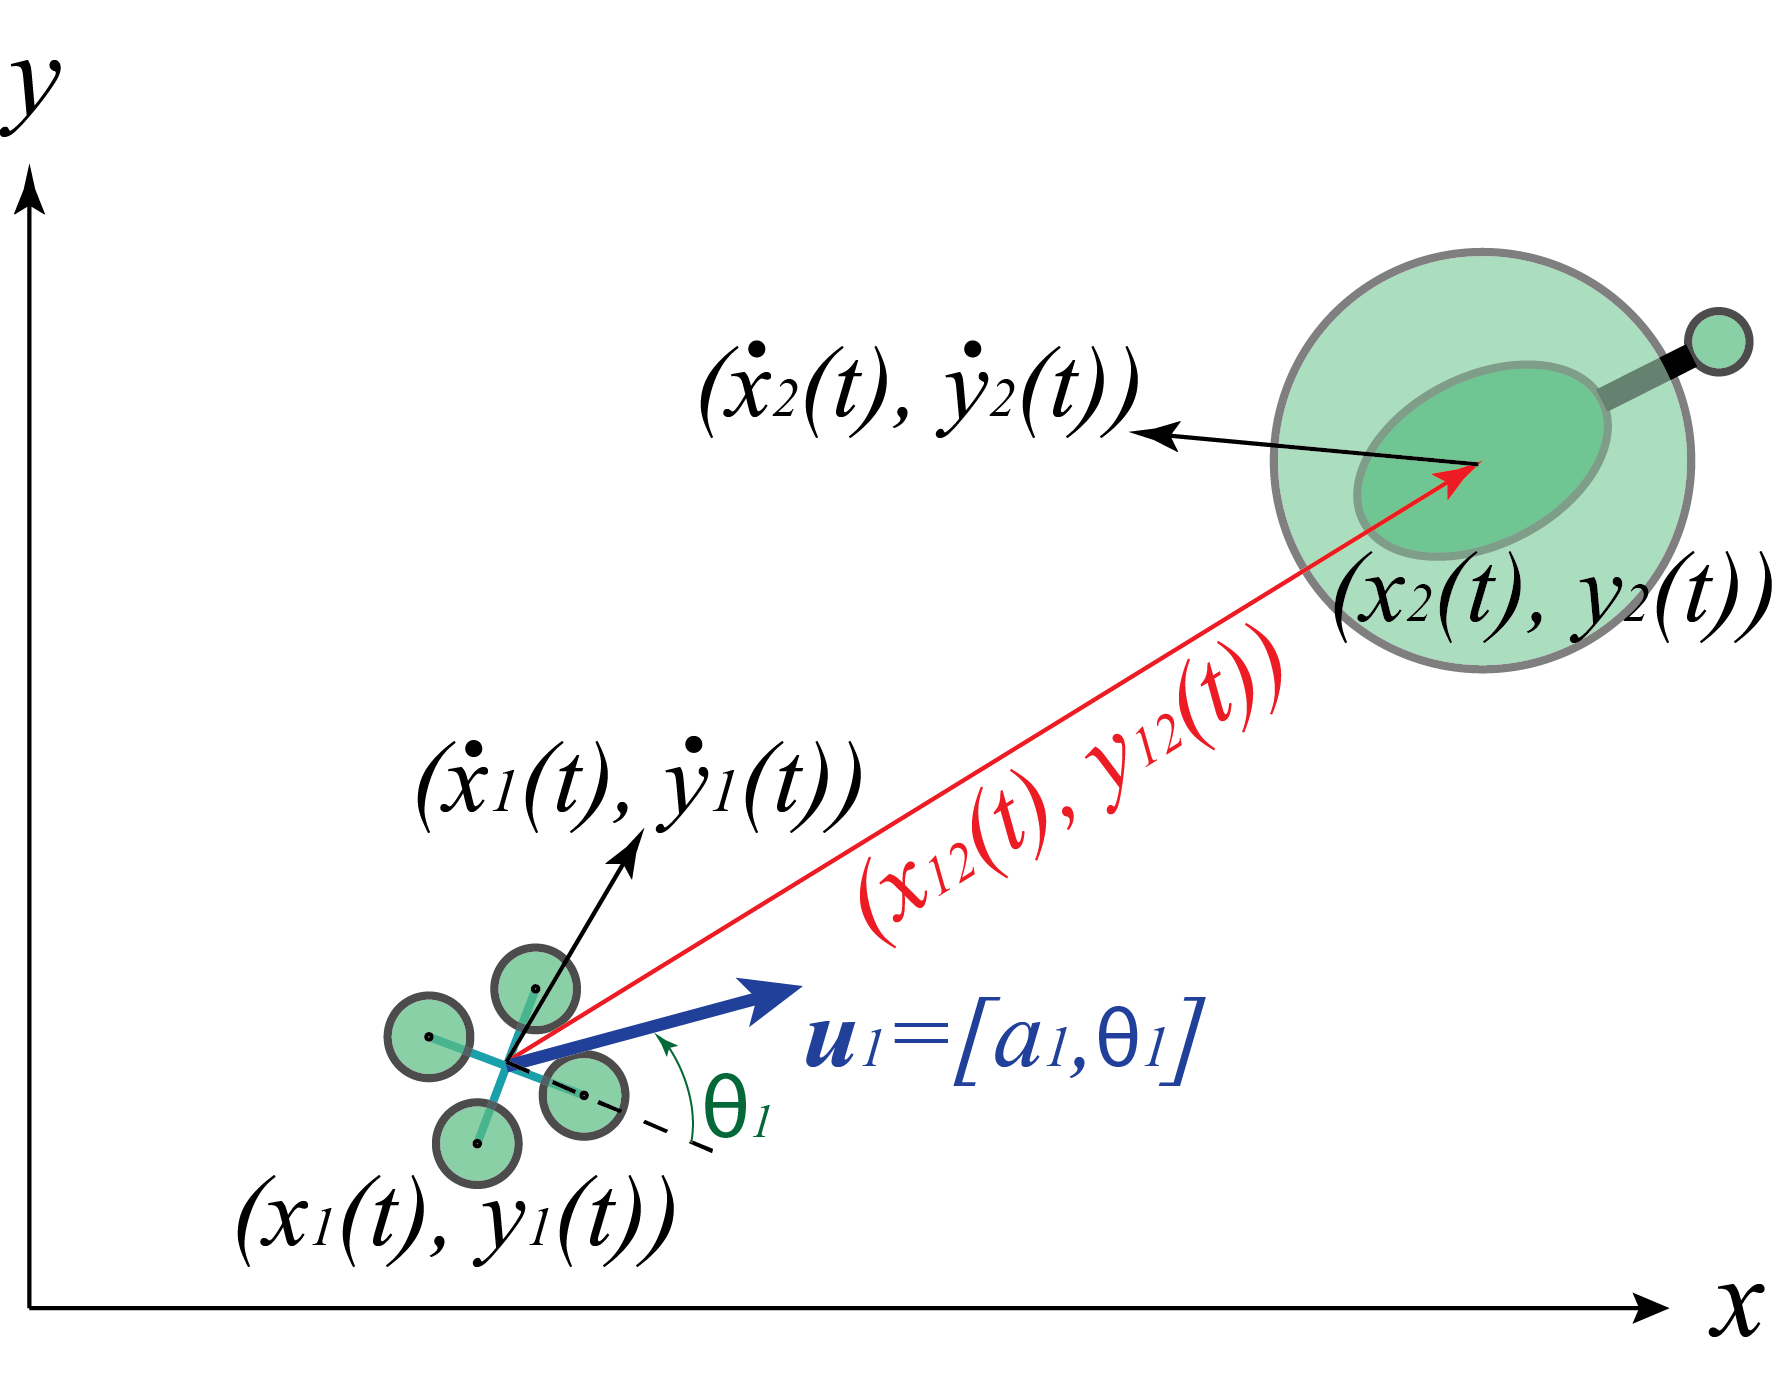
\includegraphics[width=2.5in]{problem_description}
%\caption{The collision avoidance scenario.}
%\label{fig:problem_description}
%\end{figure}

Figure \ref{fig:horiz_safety_set} highlights some position trajectories in solid red lines under optimal control. The helicopter is at the origin, and the quadrotor has a relative position $\boldsymbol{x}(t)=(x(t),y(t))$ and is heading toward the helicopter with relative velocity $\dot{\boldsymbol{x}}(t)$. The quadrotor starts the avoidance maneuver at some initial time $t=t_0$ in the past when touching the avoid set $\partial K_h$. At the present time $t=0$, the quadrotor flies tangent to the boundary of the safety set $\partial S_h$ and does not enter $S_h$.

The safety set $S_h$ is defined by the solid gray circle with radius $r_{min}$ around the quadrotor. The set of all $\boldsymbol{x}(0)$ lies on the boundary of the safety set $\partial S_h$. The quadrotor should never enter $S_h$. The set of all possible $\boldsymbol{x}(t_0)$ that come as close as possible defines the boundary of the avoid set $K_h$, indicated by the dashed red curve in Figure \ref{fig:horiz_safety_set}. The complement of $K_h$ is the maximal controlled invariant set \cite{lygeros1999controllers}, in which there is no restrictions on control. But within the avoid set $K_h$, optimal control has to be applied. Note that the relative frame is rotated such that $\dot{x} (t_0)=0$ and $\dot{y}(t_0)<0$ on $\partial K_h$. Therefore, points on $\partial K_h$ has purely downward velocities. A backward rotation should be made after the optimal control angle $\theta_h^*$ is computed \cite{hoffmann2008decentralized}.

% The WCMMD to start optimal maneuver is defined at $|\boldsymbol{x}(t_0)| \bigg|_{x(t_0)=0}$ on $\partial K_h$. 

\begin{figure}
	\centering
	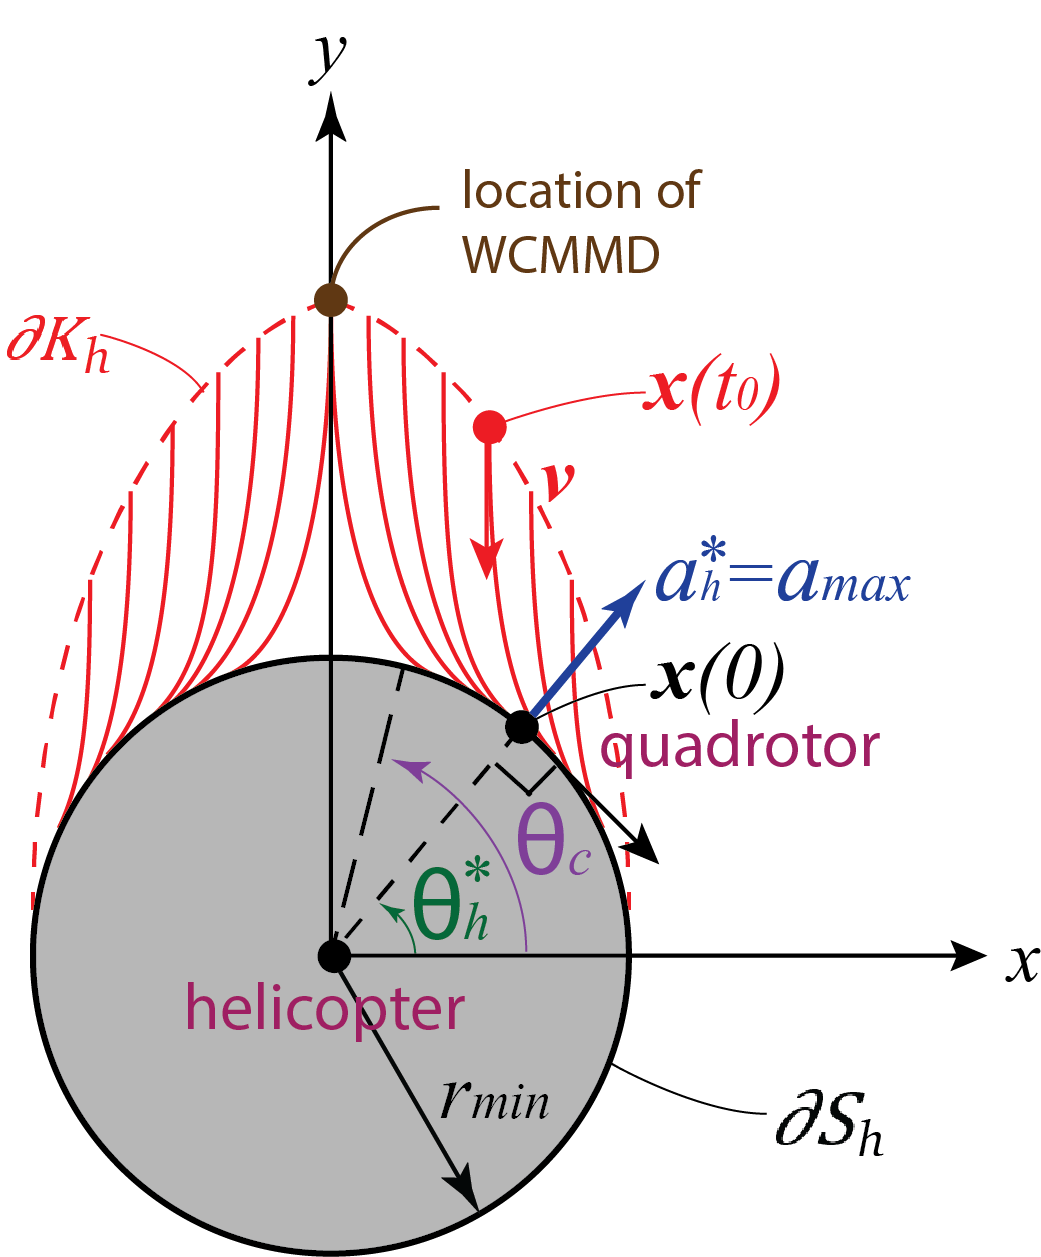
\includegraphics[width=2.5in]{horizontal_safety_set}
	\caption{The safety set $S_h$ is in gray and the avoid set $K_h$ is in red.}
	\label{fig:horiz_safety_set}
\end{figure}

Define state variables $\boldsymbol{x_h}(t)=\left[\boldsymbol{x}(t) ; \boldsymbol{\dot{x}}(t) \right]$, the relative kinematics is:

\begin{equation}
\label{eq:2D_dyn}
\begin{split}
\boldsymbol{\dot{x}_h}(t)  &= f(\boldsymbol{x_h}(t),\boldsymbol{u_h}(t)) \\
\frac{d}{dt}
\begin{bmatrix}
x(t) \\
y(t) \\
\dot{x}(t) \\
\dot{y}(t) \\
\end{bmatrix}
&=
\begin{bmatrix}
\dot{x}(t) \\
\dot{y}(t) \\
a_h(t) cos \theta_h(t) \\
a_h(t) sin \theta_h(t) \\
\end{bmatrix}
\end{split}
\end{equation}

Follow the derivation in \cite{hoffmann2008decentralized}, we obtain the optimal acceleration for $t \in [t_0,0]$ in (\ref{eq:horiz_optimal_ctrl}). 	

\begin{equation}
\label{eq:horiz_optimal_ctrl}
\begin{split}
a_h^*(t) = a_{max}; \hspace{0.5cm}
\theta_h^*(t) = atan2 \left( \frac{y(0)}{x(0)} \right) \\
\end{split}
\end{equation}


% Intuitively, $\theta_h^*$ is optimal because at this angle, all available acceleration is used to decrease the relative velocity component along the radial direction of the safety set $S_h$ at time $t=0$ (Figure \ref{fig:horiz_safety_set}). By the time the helicopter touches $\partial S_h$, this radial velocity component is zero. Consequently, the helicopter will fly with velocity $v(0)$ tangent to $\partial S_h$ and not enter $S_h$.

Then, we need to find the avoid set $\partial K_h = \{ (x(t_0), y(t_0)) \}$. It could be calculated by simple geometry. Define the relative velocity $v=|\dot{y}(t_0)|$. Given a particular $\theta_h^*$ and $r_{min}$ on $\partial S_h$,  we have

\begin{equation}
\label{eq:horiz_backward_dyn}
\begin{split}
x(t_0) &= \left( r_{min} - \frac{vsin^2\theta_h^*}{2a_{max}} \right) cos\theta_h^* \\
y(t_0) &= \left( r_{min} + \frac{v}{2a_{max}} \left( 1+cos^2\theta_h^* \right) \right) sin\theta_h^* \\
\end{split}
\end{equation}

%The derivation of  (\ref{eq:horiz_backward_dyn}) is provided in the Appendix. 

From Figure \ref{fig:horiz_safety_set}, we can see that $\theta_h^*$ is only defined on certain parts of $\partial S_h$: $\theta_h^*\in[0,\theta_c] \cup [\pi-\theta_c,\pi]$ for some $\theta_c \buildrel\triangle\over = \theta_h^* \bigg|_{x(t_0)=0}$ shown in (\ref{eq:theta_c}). At $\theta_h^*=\theta_c$ (or $x(t_0)=0$) and maximum $v$, we have the worst-case scenario, giving us the worst-case minimum maneuver distance (WCMMD) to be $y(t_0) \bigg|_{\theta_h^*=\theta_c}$ in (\ref{eq:horiz_backward_dyn}).

\begin{equation}
\label{eq:theta_c}
\begin{split}
\theta_c = sin^{-1}\frac{\sqrt{2a_{max}r_{min}}}{v}, \;\;\; 2a_{max}r_{min}<v^2
\end{split}
\end{equation}

Now we can answer the question on when to apply the optimal control. Except at $x(t_0)=0$, each point on $\partial K_h$ maps uniquely to a $\theta_h^*$ on $\partial S_h$. Therefore, we first generate $\partial K_h$ using (\ref{eq:horiz_backward_dyn}) for a dense set of $\theta_h^*\in[0,\theta_c] \cup [\pi-\theta_c,\pi]$, then compare the quadrotor's relative position $\boldsymbol{x}(t)$ to points on $\partial K_h$. If $\boldsymbol{x}(t)$  equals to a particular point on $\partial K_h$, then we can find the corresponding $\theta_h^*$ and apply  optimal acceleration $\boldsymbol{u_h^*}=[a_h^* \; \theta_h^* ]^T$. 
%Simulation proves that minimum separation distance of $r_{min}$ is indeed achieved in the simplified dynamic model (\ref{eq:2D_dyn}).

\subsection{Iterative Algorithm} \label{sec:iter_alg}

With dynamic model (\ref{eq:state_space_compact}), we can apply control (\ref{eq:horiz_optimal_ctrl}) at $\partial K_h$ defined by (\ref{eq:horiz_backward_dyn}) and (\ref{eq:theta_c}). However, the quadrotor will intrude the safety set $S_h$ due to rotational inertia and drag. To resolve the intrusion, we need to compute the worst-case earlier reaction time (WCERT), or the time the quadrotor has to react earlier before touching the safety set $S_h$, defined in Section \ref{sec:horiz_safety_controller_derivation}, to prevent collision in the worst-case scenario.

\begin{algorithm}
	\KwData{$dt$, $wcert$}
	\KwResult{$wcert$}
	\texttt{\\
		$dt$;	\hspace{3.2cm}\% time increment \\
		$wcert = 0$;	\hspace{2cm}\% current WCERT \\
		$ \boldsymbol{x}(t) = worst\_case(wcert) $\;
		\While{ $ min_t|\boldsymbol{x(t)}| < r_{min}$ }{
			$wcert = wcert + dt$\;
			$ \boldsymbol{x}(t) = worst\_case(wcert)$\;
		}
	}
	\caption{Iterative algorithm to compute WCERT.}
	\label{alg:iterative_simulation}
\end{algorithm}

Algorithm \ref{alg:iterative_simulation} computes WCERT for the horizontal safety controller. The function $ \boldsymbol{x}(t) = worst\_case(wcert) $ simulates the worst-case avoidance scenario when the kinematic controller reacts $wcert$ earlier, and return the relative horizontal position $\boldsymbol{x}(t)$ for the whole simulation period. 

We start the simulation from the safety sets (\ref{eq:horiz_backward_dyn}). If the minimum relative distance $ min_t|\boldsymbol{x(t)}|$ is less than $r_{min}$, then we increment $wcert$ and simulate again. In this case, we set $dt$ to be $0.02s$ without drag and $0.05s$ with drag, which gives a spacial resolution of $2 m$ and $5m$, respectively, when maximum speed is $v=100m/s$. 

Algorithm \ref{alg:iterative_simulation} is applied to a range of $a_{max}$ and $v$ defined in Section \ref{sec:horiz_safety_controller_derivation}. The result is a look-up table WCERT($a_{max}$,$v$). The generation of WCERT values is time-consuming but performed off line. In real flights, we can just run the light-weight kinematic safety controller in real-time but react WCERT($a_{max}$,$v$) earlier. If the dynamic model in the simulation is close to the real dynamics, then we are safe.

\subsection{Horizontal Control Conversion}
To convert the horizontal kinematic control $\boldsymbol{u_h^*}$ to dynamic controls $U_2$ and $U_3$, we assume that the quadrotor is in vertical equilibrium when performing the avoidance. The inputs that could affect the horizontal motions are the desired roll ($\phi_d$), pitch ($\theta_d$), and yaw ($\psi_d$). We choose roll and pitch since yaw is not effective. The conversion is straight forward. First, decompose the acceleration into components in the world frame $\mathcal{W}$, then rotate it to the body frame $\mathcal{B}$, and finally convert it to the desired pitch ($\theta_d$) and roll ($\phi_d$). Equation (\ref{eq:horiz_u_conversion}) summarizes the process. 

\begin{equation}
\label{eq:horiz_u_conversion}
\begin{aligned}
a_X^* &= a_{max}cos(\theta_h^*) \\
a_x^* &= cos\psi a_X + sin\psi a_Y \;\\
\theta_d &= -atan2(a_x^*,g) \\
\end{aligned}
\begin{aligned}
a_Y^* &= a_{max}sin(\theta_h^*) \\
a_y^* &= -sin\psi a_X + cos\psi a_Y \\
\phi_d &= atan2(a_y^*,g) \\
\end{aligned}
\end{equation}

\subsection{\textbf{The Hybrid Controller}}

The position controller and the safety controller together constitute a hybrid controller. The safety controller decides when the safety maneuver starts and terminates. Figure \ref{fig:hybrid_automaton} shows the hybrid automaton of the controller switching mechanism. At the beginning, the quadrotor receives a waypoint command, and the position controller starts to drive the quadrotor to the destination. When a helicopter is detected, an avoidance set calculation is performed using equation (\ref{eq:horiz_backward_dyn}). The switching occurs when $||\boldsymbol{x_{12}}(t)||_2 \le ||\boldsymbol{x_{12}}(t_0)||_2$. Once the safety controller is activated, the quadrotor avoids the helicopter by applying $a_{max}$ in the optimal direction. After $||\boldsymbol{x_{12}}(t)||_2 > ||\boldsymbol{x_{12}}(t_0)||_2$, the optimal controller is deactivated, and the quadrotor switches back to position control. If another helicopter is passing by, the optimal control is enabled again.

\begin{figure}
\centering
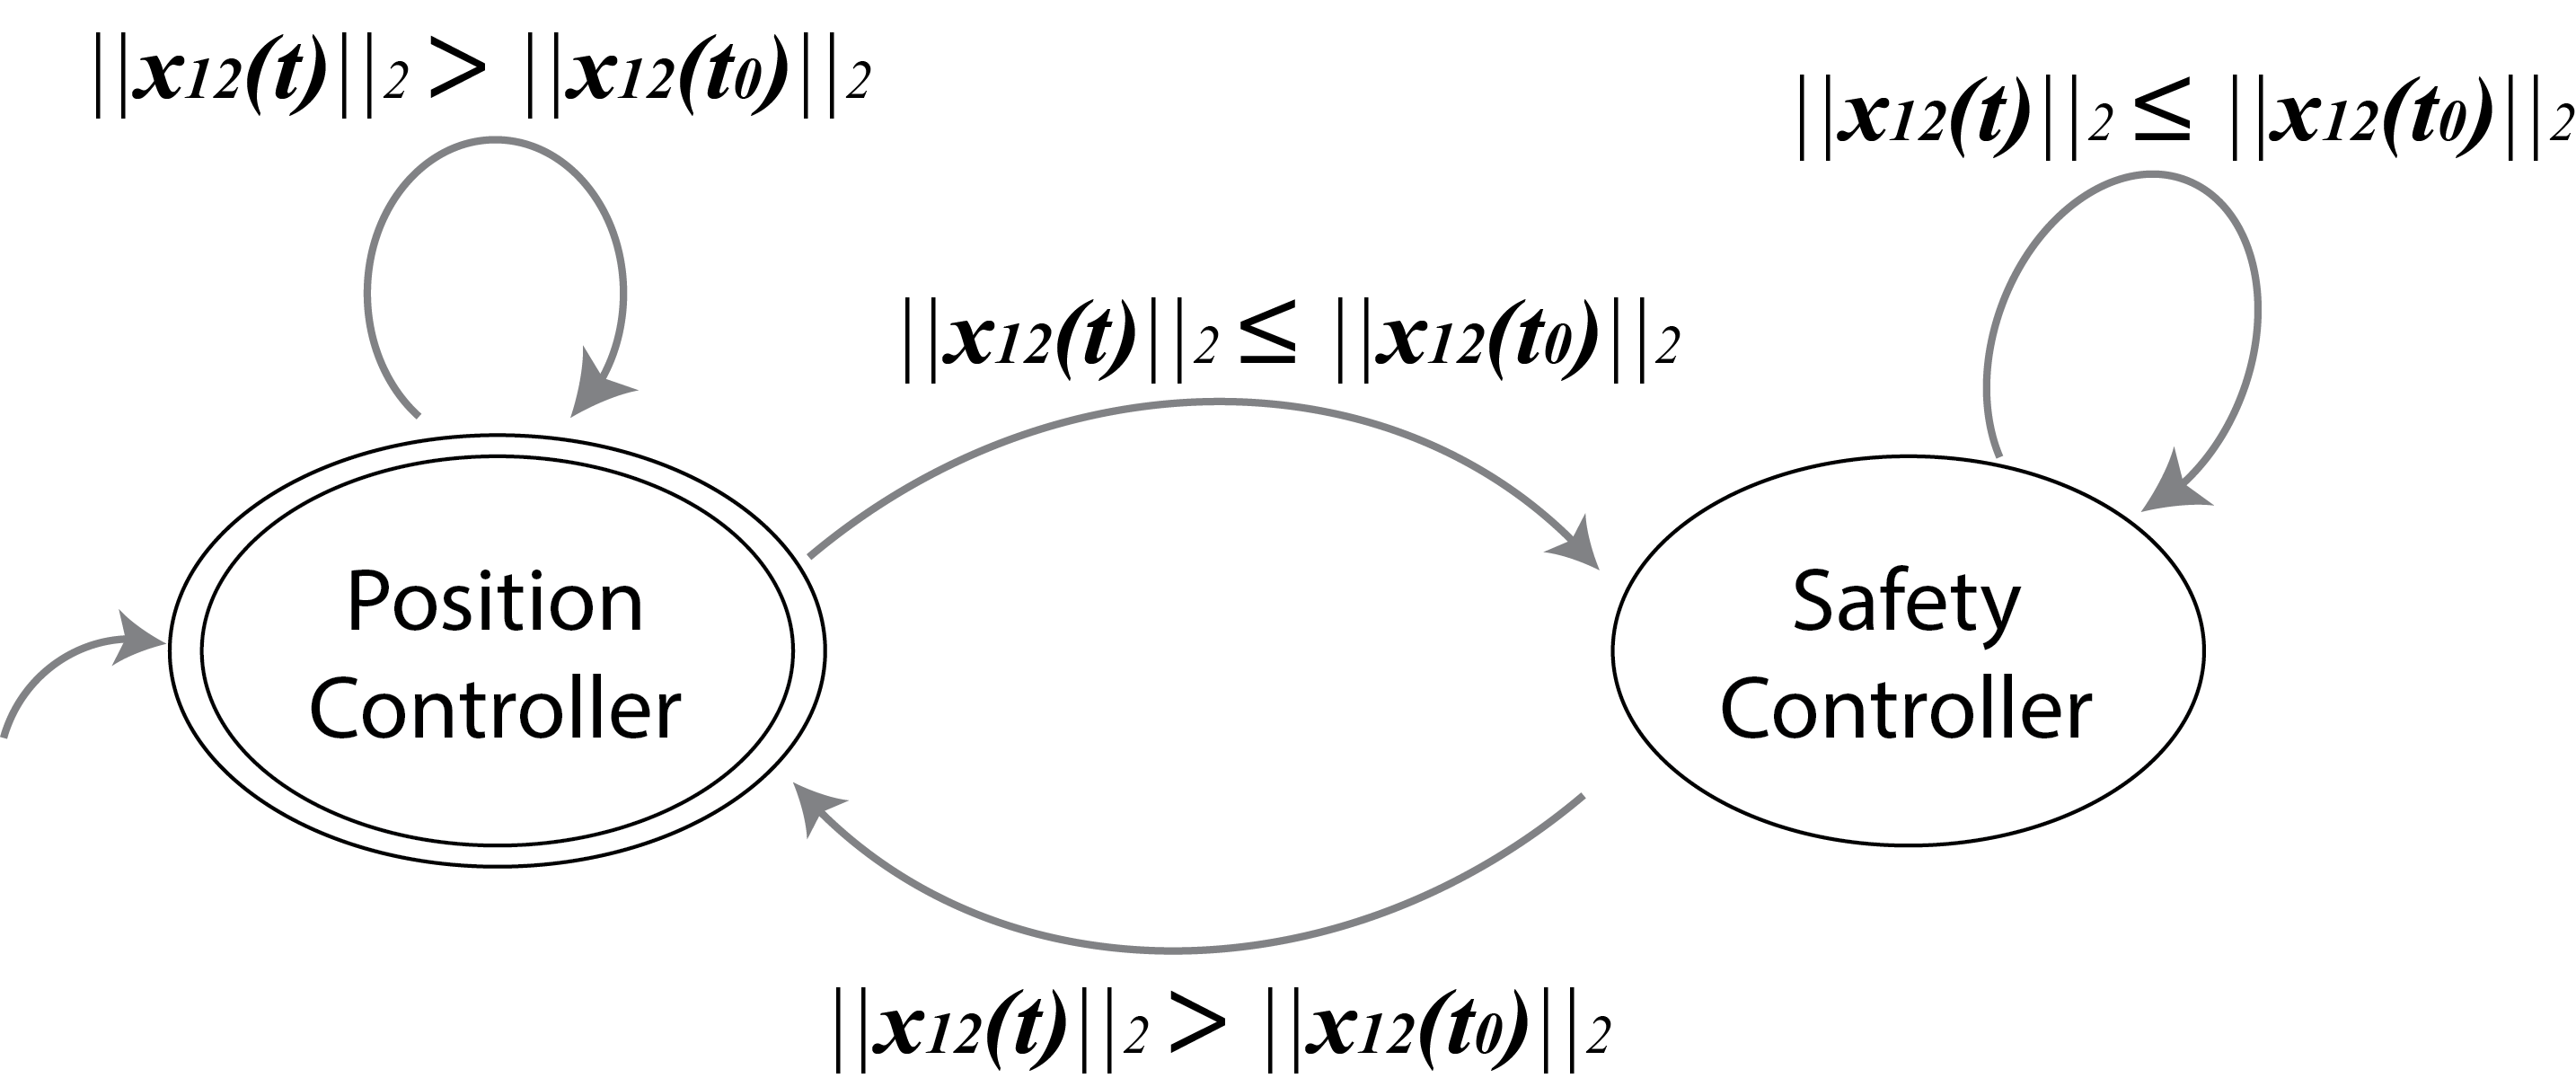
\includegraphics[width=3in]{hybrid_automaton}
\caption{The hybrid automaton indicating the controller switching mechanism.}
\label{fig:hybrid_automaton}
\end{figure}

\section{\textbf{Simulation}} \label{sec:simulation}


In this paper, we use the parameters in equation (\ref{eq:model_param}) to mimic a realistic model (3DR Solo \cite{3dr_solo}), whose weight and capability are similar to most of the quadrotors sold in the market today. We choose conservative parameter values carefully. There are three uncertain key parameters which dominates the simulation results, namely the rotational inertia (RI) $I$, the translation drag coefficient $c_t$, and the communication delay $\Delta t_{delay}$. Refer to Section \ref{sec:dynamic_model} for the variables.

\begin{equation}
\label{eq:model_param}
\begin{aligned}
m &= 1.5 \; kg \\
k_m &= 10^{-6} \; Nm \cdot s^2 \;\;\; \\
c_t &=  0.50 \; Ns/m \;\;\;\\
l &= 0.2 m \\
\end{aligned}
\begin{aligned}
I &= diag([5 \; 5 \; 8]e\text{-}3) \; kg \cdot m^2 \\
k_f &= 5.0 \times 10^{-6} \; N \cdot s^2 \\
c_r &= 0.10 \; Nm \cdot s^2 \\
\boldsymbol{g} &= \left[0 \; 0\; 9.81 \right]^T \; m/s^2 \\
\end{aligned}
\end{equation}

\begin{itemize}
	\item $\boldsymbol{I}=diag(I_x,I_y,I_z)$: We approximate the rotational inertia (RI) by approximating the 3DR Solo as a solid cylinder of radius $0.1m$ and height $0.1m$. The calculation follows from \cite{beer1972statics}, and the system identification results in \cite{bouadi2011adaptive} validates our calculation.
	
	\item $c_t$: Instead of adopting results from \cite{bouadi2011adaptive}, which yields an unrealistically large terminal velocity, we picked a more conservative value of $0.5 Ns/m$ from [\citen{dragcoeff}, \citen{munson1990fundamentals}]. The number is validated from static equilibrium between maximum horizontal thrust of $\sqrt{3}mg$ and translation drag $c_t v_{max}$, where $v_{max}=50m/s$ is the terminal speed of the quadrotor \cite{quadrotor_common_speed}.
	
	\item $\Delta t_{delay}$: The communication delay is set to $1.0 s$ throughout the simulations, to approximate the worst-case behavior of ADS-B \cite{helfrick2010principles}.
\end{itemize}

The simulation is expected to be realistic, although a hardware implementation is necessary to confirm the effectiveness of the hybrid controller. However, the hardware implementation is too involved, and thus not presented at this stage. It will be left as future work.

\subsection{Safety Controller} \label{sec:safety_controller_result}

In this section, two set of simulation results are presented. First, we examine how the 2D safety controller behaves when applied to the full 3D quadrotor model. Then, we present the WCMMD and WCERT results covering all practical cases in heatmaps. All safety sets are produced by griding $120$ points evenly for $\theta_h^*\in[0,\theta_c] \cup [\pi-\theta_c,\pi]$.

\subsubsection{safety controller behavior}

Figure \ref{fig:roll_pitch_avoidance} shows the behavior of the safety controller. Two factors, namely the magnitude of the maximum acceleration and drag force, are investigated. The dashed red lines are the reference signals generated from the high-level safety controller, while the black solid lines are the tracking signals from the low-level sliding mode angle controllers \cite{bouadi2011adaptive}. The quadrotor is originally at rest. The parameters are

\begin{equation*}
\label{eq:safety_param}
\begin{split}
\begin{matrix}
a_{max} = \left[ 2 \; 5 \; 10 \right] m/s^2 \;\;\;\;\;\;\;\;&
r_{min} = 20m \;\;\;\;\;\;\;\;&
v_{12} = 70m/s \\
\end{matrix}
\end{split}
\end{equation*}

\begin{figure}
    \centering
    \begin{subfigure}{.47\columnwidth}
        \centering
        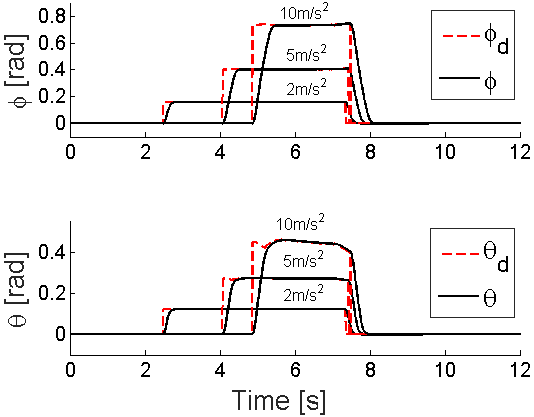
\includegraphics[width=\columnwidth]{roll_pitch_avoidance}
        \caption{without drag force}
        \label{fig:roll_pitch_avoidance_frictionless}
    \end{subfigure}
    \hfill
    \begin{subfigure}{.47\columnwidth}
        \centering
        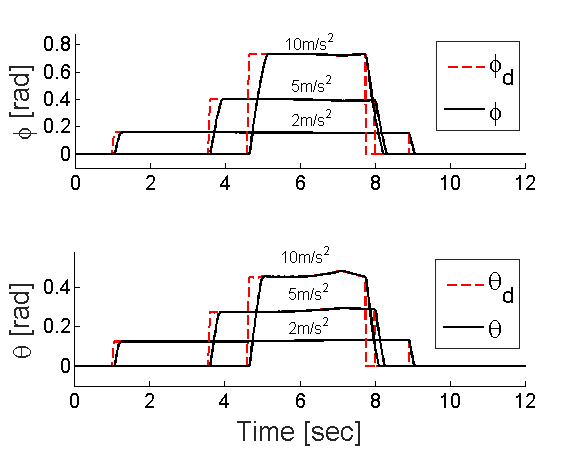
\includegraphics[width=\columnwidth]{roll_pitch_avoidance_friction}
        \caption{with drag force}
        \label{fig:roll_pitch_avoidance_friction}
    \end{subfigure}
    \caption{The 
    2D optimal safety control is applied to a 3D quadrotor model.}
    \label{fig:roll_pitch_avoidance}
\end{figure}

In Figure \ref{fig:roll_pitch_avoidance_frictionless}, when $a_{max}$ is low, say $2m/s^2$, the constant acceleration assumption holds very well, but in sacrifice it takes a long time ($4.9 s$) to finish the avoidance maneuver. At the beginning of the avoidance maneuver, the tracking delay between the dashed red line and the solid black line is $0.28s$, which results in a ERT of $0.1s$.

The avoidance duration is shortened to half as much ($2.6 s$) when $a_{max}=10m/s^2$, but the desired pitch $\theta_d$ has some variation at the beginning and the end of the avoidance. The variation exists because the quadrotor could not achieve the desired acceleration instantaneously due to rotational inertia (RI). Nonetheless, the assumption of applying constant maximum acceleration remains valid. The tracking delay is $0.56s$, which gives a ERT of $0.2s$. When $a_{max}=5m/s^2$, the result is somewhere in between. As $a_{max}$ increases, the tracking delay increases, and ERT increases almost propotional to the tracking delay. Therefore, without drag, ERT is solely determined by the tracking delay at the beginning of the avoidance maneuver.

In the normal case with drag force (Figure \ref{fig:roll_pitch_avoidance_friction}), the variation in desired pitch ($\theta_d$) is worse, although the desired roll ($\phi_d$) stays almost constant. $\theta_d$ is generally increasing during the avoidance maneuver, especially at $a_{max}=10m/s^2$. It makes sense because as the velocity goes up, the drag force goes up, and to generate an equivalent $a_{max}$, a larger pitch angle is needed. The avoidance duration is longer, range from $7.9s$ (when $a_{max}=2m/s^2$) to $3.1s$ (when $a_{max}=10m/s^2$).

However, with drag, ERT is not a strong function of tracking delay anymore. With similar tracking delays, the ERT is $1.54s$ when $a_{max}=2m/s^2$ and $0.42s$ when $a_{max}=10m/s^2$. This result is the complete opposite to the no-drag case. As $a_{max}$ increases, the drag force increases faster, and to counteract the drag, a larger ERT is required.


\subsubsection{worst-case scenarios}

In this section, we discuss the simulation results of the safety controller in Section \ref{sec:horiz_safety_controller_derivation}. The WCMMD and WCERT, defined in Section \ref{sec:horiz_safety_controller_derivation}, are observed when the quadrotor and helicopter are heading directly to each other at maximum horizontal relative velocity at the same altitude. The effect of rotational inertia (RI), drag forces, and communication delay described in Section \ref{sec:simulation} are evaluated.

\begin{figure}
	\centering
	\begin{subfigure}{.45\columnwidth}\centering%no!\hfill
		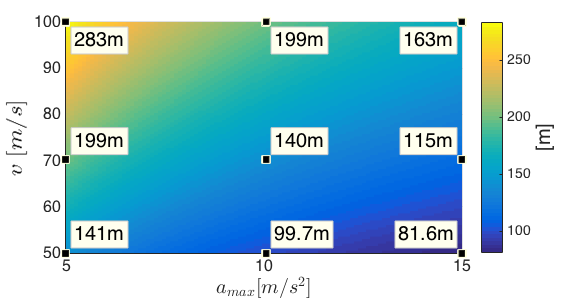
\includegraphics[width=\columnwidth]{WCMMD_horizontal_kinematics}
		\caption{kinematics only}
		\label{fig:WCMMD_horiz_kinematics}
	\end{subfigure}%
	\hfill
	\begin{subfigure}{.45\columnwidth}\centering
		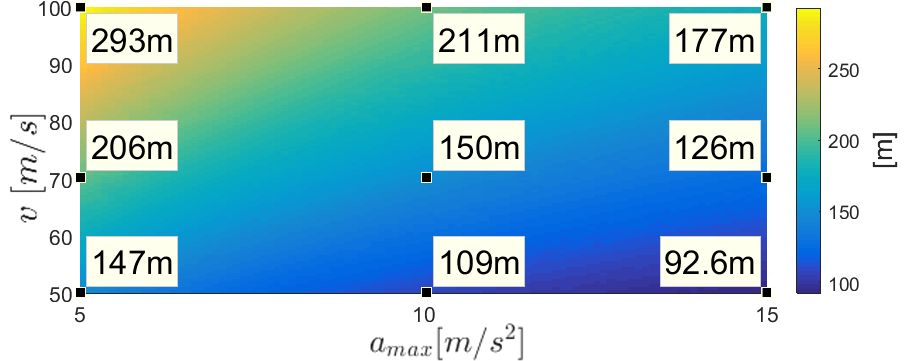
\includegraphics[width=\columnwidth]{WCMMD_horizontal_RI}
		\caption{with RI}
		\label{fig:WCMMD_horiz_RI}
	\end{subfigure}%
	\hfill
	\begin{subfigure}{.45\columnwidth}\centering
		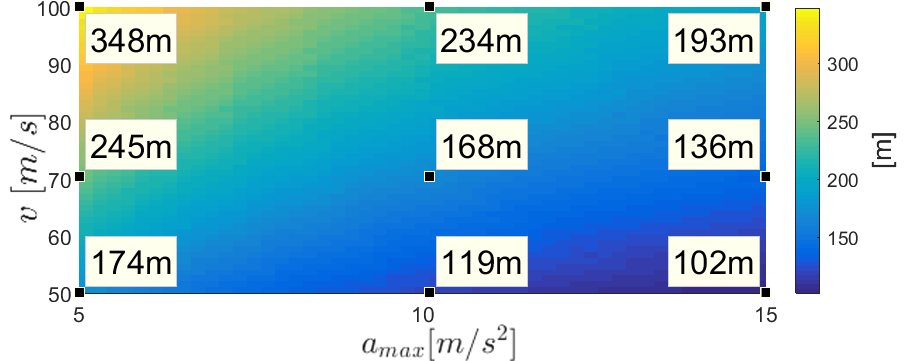
\includegraphics[width=\columnwidth]{WCMMD_horizontal_RI_drag}
		\caption{with RI and drag}
		\label{fig:WCMMD_horiz_RI_drag}
	\end{subfigure}%
	\hfill
	\begin{subfigure}{.45\columnwidth}\centering
		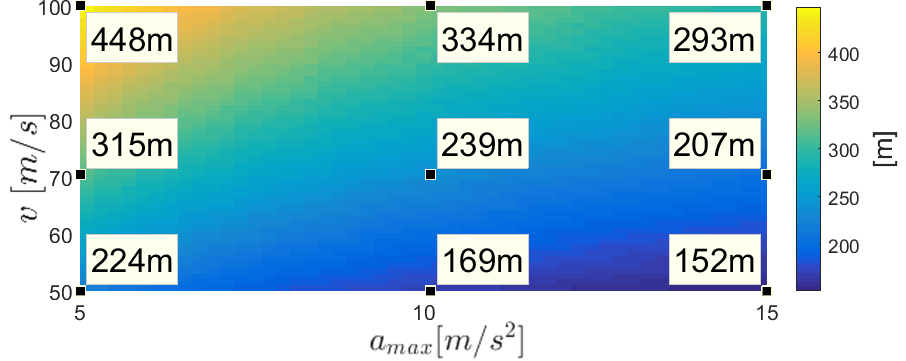
\includegraphics[width=\columnwidth]{WCMMD_horizontal_RI_drag_delay}
		\caption{with RI, drag, and comm. delay}
		\label{fig:WCMMD_horiz_RI_drag_delay}
	\end{subfigure}%
	\caption{Summary of WCMMD for the horizontal controller ($r_{min}=20m$).}
\end{figure}

Figure \ref{fig:WCMMD_horiz_kinematics} shows the WCMMD result by using the horizontal safety controller on a kinematic quadrotor. It serves as the base of comparison. The ranges for $a_{max}$ and $v$ are chosen for reasons. A quadrotor can typically produce a maximum thrust of twice as its weight, or $2mg$ \cite{quad_design}, which can generate a maximum horizontal acceleration of $17m/s^2$ when tilting at $60^{\circ}$ at a constant altitude. Therefore, we picked $a_{max}$ to be between $5$ and $15m/s^2$. A commercial helicopter typically has a maximum horizontal speed of $70m/s$ \cite{helicopter_common_speed}, while a quadrotor has a maximum cruise speed of $30m/s$ \cite{quadrotor_common_speed}. Therefore, we set the maximum horizontal relative velocity $v$ to be between $50$ and $100m/s$.

Figure \ref{fig:WCMMD_horiz_RI}, \ref{fig:WCMMD_horiz_RI_drag}, and \ref{fig:WCMMD_horiz_RI_drag_delay} give the WCMMD results by using the horizontal safety controller on a quadrotor with RI, drag, and communication delay, respectively. The axis ranges are the same as Figure \ref{fig:WCMMD_horiz_kinematics} for comparison purpose.

The WCMMD increases faster and faster from the lower-right corner to the upper-left corner. In the lower-right corner, when $a_{max}$ is high and $v$ is low, we get small WCMMD ranging from $93 m$ (no drag) to $152 m$ (with drag and communication delay). In the upper-left corner, with small $a_{max}$ and large $v$, we get large WCMMD ranging from $293 m$ to $448 m$. Compared with Figure \ref{fig:WCMMD_horiz_kinematics}, RI gives a maximum of $10 m$, or $3\%$, increase in the WCMMD. The WCMMD increments due to drag are $55 m$, or $18\%$, in the upper left corner and $10 m$, or $10\%$, in the lower right corner. Lastly, depending on the relative velocity $v$, the WCMMD increment of communication delay range from $50 m$ ($15\%$) to $100 m$ ($30\%$).

\begin{figure}
	\centering
	\begin{subfigure}{.48\columnwidth}
		\centering
		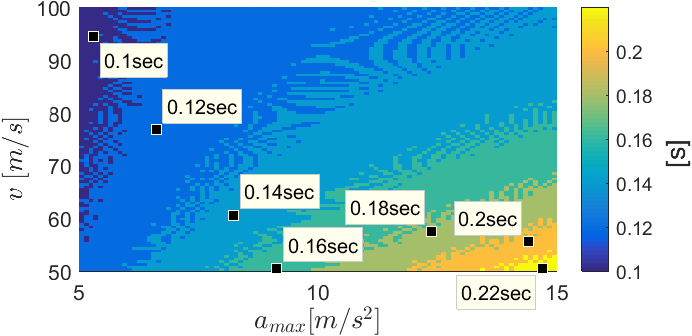
\includegraphics[width=\columnwidth]{WCERT_horizontal_RI}
		\caption{with RI}
		\label{fig:WCERT_horiz_RI}
	\end{subfigure}
	\hfill
	\begin{subfigure}{.48\columnwidth}
		\centering
		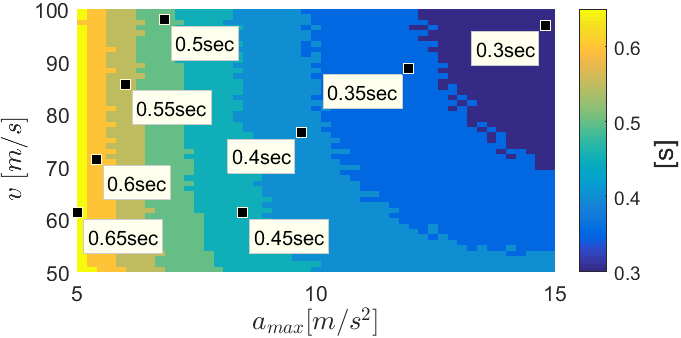
\includegraphics[width=\columnwidth]{WCERT_horizontal_RI_drag}
		\caption{with RI and drag}
		\label{fig:WCERT_horiz_RI_drag}
	\end{subfigure}
	\caption{Summary for the
		WCERT as defined in Section \ref{sec:horiz_safety_controller_derivation} ($r_{min}=20m$).}
	\label{fig:WCERT_horiz}
\end{figure}

The more interesting result comes in the WCERT maps. First, the WCERT values without drag is always smaller than the ones with drag. The WCERT ranges from $0.10 s$ to $0.22 s$ without drag and from $0.30 s$ to $0.65 s$ with drag. Second, the two WCERT maps in Figure \ref{fig:WCERT_horiz} show opposite patterns with respect to $a_{max}$. With RI only (Figure \ref{fig:WCERT_horiz_RI}), the WCERT increase as $a_{max}$ increases. It is because a larger $a_{max}$ implies a larger tilting angle ($\phi_d$ and $\theta_d$), which takes more time for the sliding mode controllers to rotate the quadrotor. With both RI and drag (Figure \ref{fig:WCERT_horiz_RI_drag}), the WCERT decreases as $a_{max}$ increases. It says that as $a_{max}$ gets larger, it becomes easier to overcome the drag, and the WCERT becomes smaller. To take into account the communication delay, one can simply add the delay ($1s$ for ADS-B) on top of Figure \ref{fig:WCERT_horiz}.

\subsection{Hybrid Controller}

We tested the hybrid controller extensively in a wide range of scenarios to prove its effectiveness. Here we only present a typical package-delivery scenario. A quadrotor is typically designed to produce a maximum thrust of $2mg$ \cite{quad_design}, which can give a maximum horizontal acceleration of $14m/s^2$ when hovering. Figure \ref{fig:waypoint_avoidance} shows a high-speed high-acceleration scenario. In Figure \ref{fig:trajectory}, the quadrotor takes off from the origin and is trying to get to the point $(X,\;Y, \; Z)=(500m, \; 500m, \; \text{-}100m)$ when a helicopter is flying toward it in a straight line. The horizontal position signals of both the helicopter and the quadrotor are contaminated with Gaussian white noise with a standard deviation of $5m$. In addition, the quadrotor is experiencing a horizontal wind disturbance of $\boldsymbol{V_{wind}}$ similar to \cite{madani2006backstepping_2}. In this scenario, the parameters are

\begin{equation*}
\label{eq:hybrid_param}
\begin{split}
\begin{matrix}
r_{min} = 20 m &
a_{max} = 14 m/s^2 &
\boldsymbol{V_{wind}}=[\text{-}10, \; \text{-}10,\; 0]m/s\\
v_{heli} = 70 m/s &
v_{quad} = 28.3 m/s &
v_{12} = 98.3 m/s \\
\end{matrix}
\end{split}
\end{equation*}

\begin{figure}
	\centering
	\begin{subfigure}[b]{0.35\columnwidth}
		\centering
		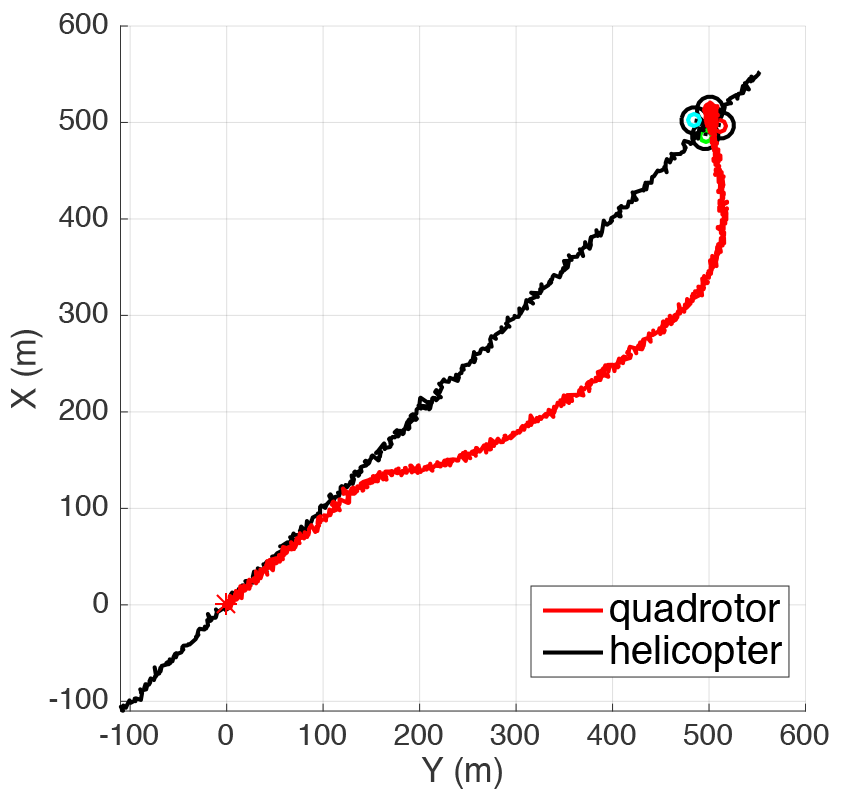
\includegraphics[width=\columnwidth]{trajectory}
		\caption{horizontal position trajectory}
		\label{fig:trajectory}
	\end{subfigure}
	\hfill
	\begin{subfigure}[b]{0.64\columnwidth}
		\centering
		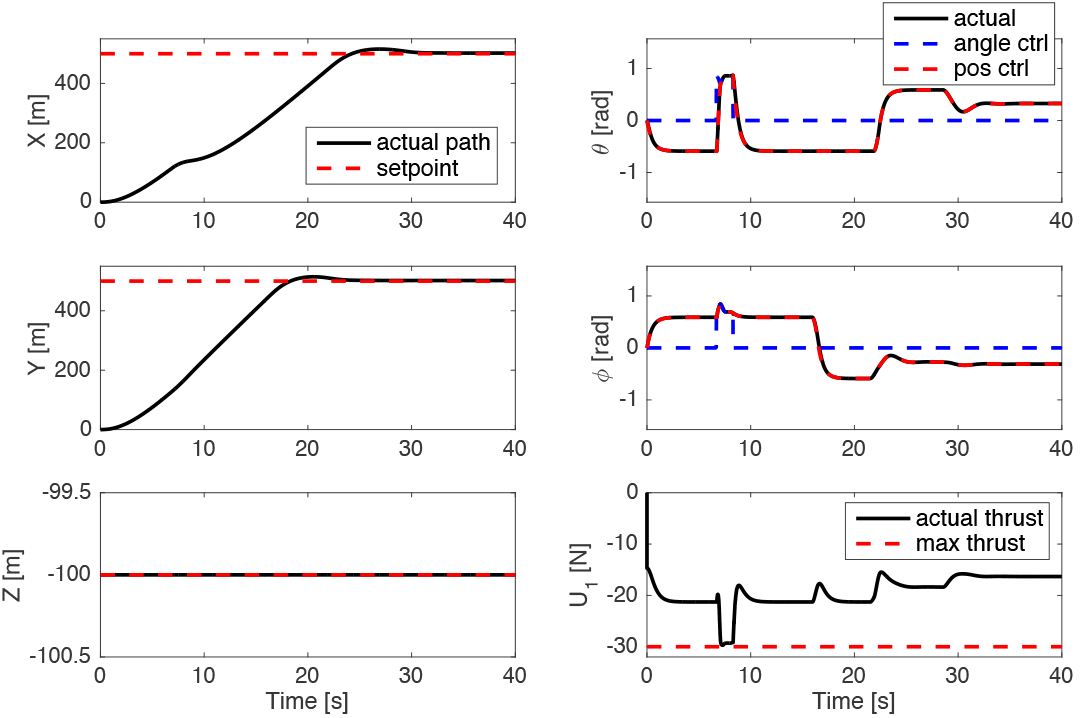
\includegraphics[width=\columnwidth]{tracking}
		\caption{time history of reference and control signals.}
		\label{fig:tracking}
	\end{subfigure}
	
	\caption{The quadrotor avoids a helicopter on the way to a destination.}
	\label{fig:waypoint_avoidance}
\end{figure}

By employing the safety controller, the quadrotor successfully avoids the helicopter and gets to the final destination (Figure \ref{fig:trajectory}). Assume that there is no communication delay, when the WCERT is set to $0.1s$, the minimum relative distance between the two vehicles is $r_{12,min}=21.8m$, which is barely larger than the nominal threshold $r_{min}=20m$, indicating that the safety controller performs almost optimally. Note that if the vehicles are equipped with ADS-B, the WCERT should take into account the $1s$ communication delay, giving a WCERT value of $1.1s$.

Figure \ref{fig:tracking} shows the time history of the horizontal command and control signals. In all subplots, the black solid lines give the actual signal trajectory. In the $X$, $Y$, and $Z$ time history plots, the red dashed lines indicate desired destination. In the $\theta$ and $\phi$ plots, the blue dashed lines show the command generated from the angle (safety) controller, and the red dashed lines give command from the position controller. At the beginning, position control is enabled, and the actual trajectory (solid black) follow the position control command. At time $t=6.7s$, the quadrotor switches to the safety control until $t=8.3s$, which gives an avoidance duration of $1.6s$. The tracking delay in roll ($\phi$) is long ($\sim 0.44s$) since the error between the desired roll and the actual roll is large at the beginning of the avoidance. During the safety avoidance, the quadrotor is under angle control, and the position control signal $X_d$ and $Y_d$ follow the actual position $X$ and $Y$, instead. After the safety maneuver, the quadrotor switches back to position control smoothly. After arriving at the destination ($t \ge 32 s$), the quadrotor still has nonzero roll and pitch to counteract the wind disturbance. Note that full thrust ($U_1$) is applied during the avoidance, indicating the choice of $a_{max}$ is the highest achievable acceleration. Nonetheless, the quadrotor goes to the destination quickly in $27.5 s$, indicating that effectiveness of the sliding mode controllers, even in presence of wind disturbance and measurement noise.

The efficiency of the safety controller could also be evaluated by the total flight time. In this scenario, if the quadrotor were flying straight without the helicopter, the total flight time would be $27.5 s$, and that with avoidance is $31.8 s$, which gives an overall navigation delay of $4.3 s$. After deducting the $1.6 s$ avoidance maneuver, the navigation time is increased by $2.7 s$. If the destination is $10$ miles away, the total flight time would be around $10$ minutes. The navigation delay ($4.3 s$) gives a $0.7\%$ increase in the total flight time. The optimality ensures that the extra time spent on avoidance is not significant compared to the whole trip.



%\begin{figure*}[!t]
%%\normalsize 		% ensure that we have normalsize text
%\begingroup\makeatletter\def\f@size{8}\check@mathfonts
%\begin{equation}
%\label{eq:state-space_expanded}
%\begin{split}
%\begin{bmatrix}
%\dot{X}\\ 
%\dot{Y}\\ 
%\dot{Z}\\ 
%\dot{\phi}\\ 
%\dot{\theta}\\ 
%\dot{\psi}\\ 
%\dot{V}_X\\ 
%\dot{V}_Y\\ 
%\dot{V}_Z\\ 
%\dot{\omega}_x\\ 
%\dot{\omega}_y\\ 
%\dot{\omega}_z
%\end{bmatrix}
%=
%\begin{bmatrix}
%V_X\\ 
%V_Y\\ 
%V_Z\\ 
%\omega_x+\omega_y sin\phi tan\theta+\omega_z cos\phi tan\theta\\ 
%\omega_ycos\phi-\omega_z sin\phi\\ 
%-\frac{c_t}{m}V_X\\ 
%-\frac{c_t}{m}V_Y\\ 
%-\frac{c_t}{m}V_Z\\ 
%\frac{I_y-I_z}{I_x}\omega_y \omega_z - \frac{c_r}{I_x}\omega_x^2-\frac{I_r}{I_x} \Omega\omega_y \\
%\frac{I_z-I_x}{I_y}\omega_x \omega_z - \frac{c_r}{I_y}\omega_y^2-\frac{I_r}{I_y} \Omega\omega_x \\ 
%\frac{I_x-I_y}{I_x}\omega_x \omega_y - \frac{c_r}{I_z}\omega_z^2 \\ 
%\end{bmatrix}
%+
%\begin{bmatrix}
%0 \\0 \\ 0\\ 0\\ 0\\ 0\\ 
%\frac{cos\phi sin\theta cos\psi + sin\phi sin\psi}{m} \\ 
%\frac{cos\phi sin\theta sin\psi - sin\phi cos\psi}{m} \\ 
%\frac{cos\phi cos\theta}{m} \\ 
%0 \\0 \\ 0
%\end{bmatrix}
%U_1+
%\begin{bmatrix}
%0\\ 0\\ 0\\ 0\\ 0\\ 0\\ 0\\ 0\\ 0\\ \frac{l}{I_x}\\ 0\\ 0
%\end{bmatrix}
%U_2+
%\begin{bmatrix}
%0\\ 0\\ 0\\ 0\\ 0\\ 0\\ 0\\ 0\\ 0\\ 0\\ \frac{l}{I_y}\\ 0
%\end{bmatrix}
%U_3+
%\begin{bmatrix}
%0\\ 0\\ 0\\ 0\\ 0\\ 0\\ 0\\ 0\\ 0\\ 0\\ 0\\ \frac{1}{I_z}
%\end{bmatrix}
%U_4
%\end{split}
%\end{equation}
%\endgroup
%\end{figure*}

\section{\textbf{Conclusion}}

In this paper, a hybrid controller with collision avoidance capability is presented in the context of high-speed quadrotor-helicopter flights. A concise position controller is formulated by adopting DSC techniques. In addition, a computationally feasible optimal safety controller is proposed for a 3D quadrotor. The combined hybrid controller is capable of performing optimal avoidance in autonomous navigation.

Some future work remains. First, the safety controller should be improved to handle a small multi-helicopter avoidance scenario. Second, the hybrid controller should be integrated with a path following algorithm, which is necessary to avoid multi-drone-to-drone collision in air highways. Lastly, a hardware implementation is necessary to confirm its effectiveness in real life.

%\appendices
%\section*{Appendix}
%
%Figure \ref{fig:backward_dynamics} shows the trajectory from $\left( x_{12}(t_0) , y_{12}(t_0) \right)$ to $\left( x_{12}(0) , y_{12}(0) \right)$. Decompose the trajectory along and perpendicular to the direction of $\theta_1^*$ into $d_1$ and $d_2$. Given the initial speed $v_i = v_{12}(t_0)sin\theta_1^*$, final speed $v_f = 0$, and the constant external force $-ma_{max}$, we have 
%
%\begin{equation*}
%\label{eq:derivation1}
%\begin{split}
%d_1 &= \frac{\left(v_{12}(t_0)sin\theta_1^*\right)^2}{2a_{max}} \\
%d_2 &= \left(v_{12}(t_0)cos\theta_1^*\right) \left( \frac{v_{12}(t_0)sin\theta_1^*}{2a_{max}} \right) \\
%\end{split}
%\end{equation*}
%
%Lastly, by geometry,
%
%\begin{equation*}
%\label{eq:derivation2}
%\begin{split}
%x_{12}(t_0) - d_1 cos\theta_1^* + d_2 sin\theta_1^* &= r_{min}cos\theta_1^* \\
%y_{12}(t_0) - d_1 sin\theta_1^* - d_2 cos\theta_1^* &= r_{min}sin\theta_1^* \\
%\end{split}
%\end{equation*}
%
%which results in (\ref{eq:backward_dyn}).
%
%
%\begin{figure}
%\centering
%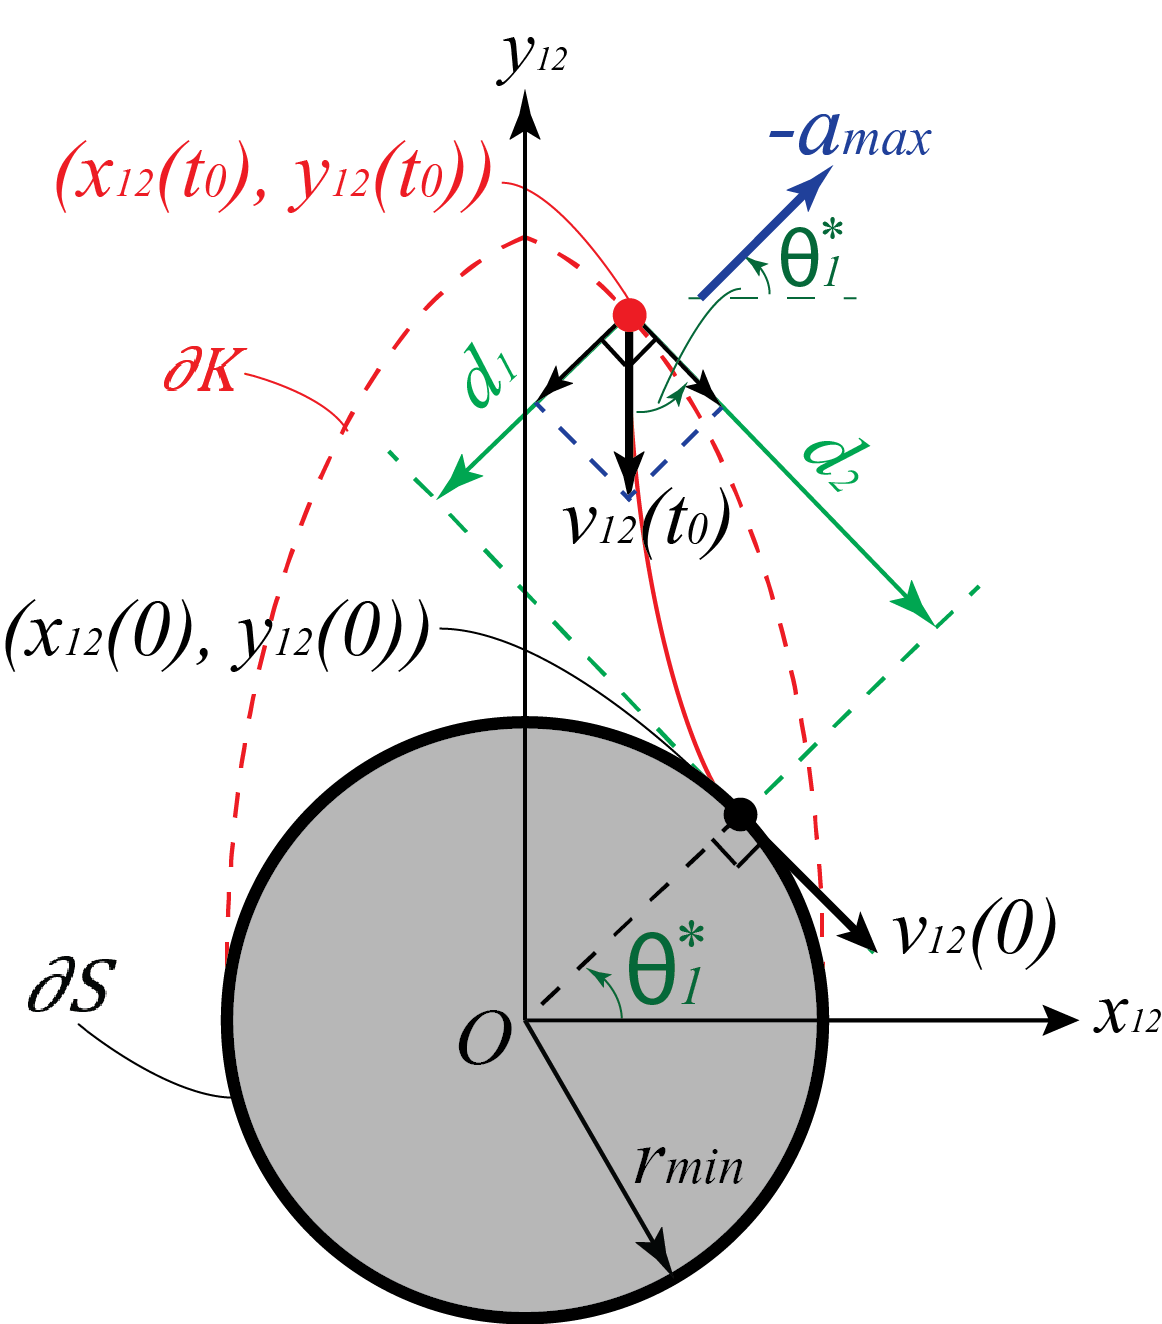
\includegraphics[width=2.5in]{backward_dynamics}
%\caption{Backward dynamics diagram.}
%\label{fig:backward_dynamics}
%\end{figure}


%\begin{figure*}
%    \centering
%    \begin{subfigure}[b]{0.475\textwidth}
%        \centering
%        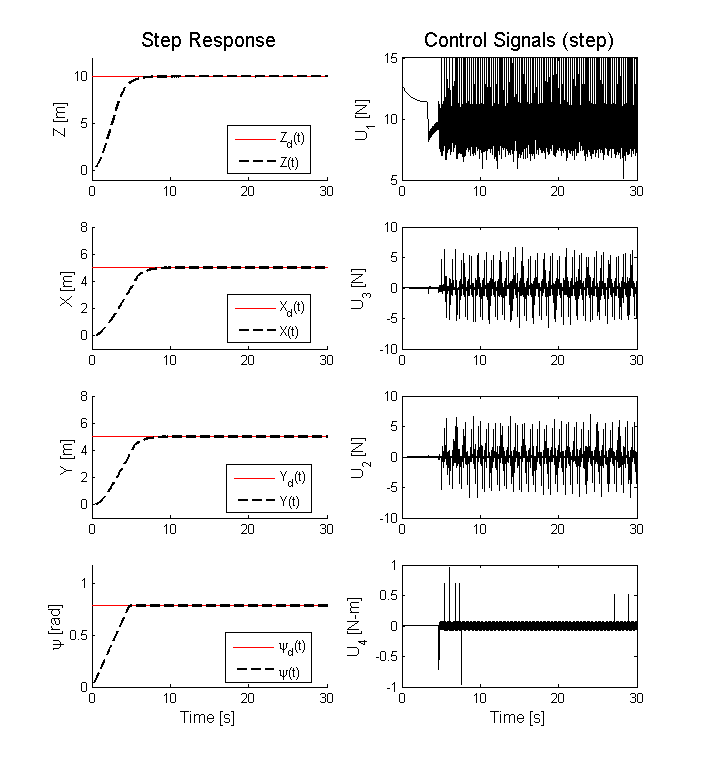
\includegraphics[width=\textwidth]{chattering_SM}
%        \caption[]%
%        {{sliding mode}}    
%        \label{fig:sliding_mode}
%    \end{subfigure}
%    \hfill
%    \begin{subfigure}[b]{0.475\textwidth}  
%        \centering 
%        \includegraphics[width=\textwidth]{tracking_SM_sat_smooth}
%        \caption[]%
%        {{sliding with saturation smoothing}}    
%        \label{fig:sliding_sat}
%    \end{subfigure}
%    \vskip\baselineskip
%    \begin{subfigure}[b]{0.475\textwidth}   
%        \centering 
%        \includegraphics[width=\textwidth]{tracking_SM_exp_smooth}
%        \caption[]%
%        {{sliding with logistical smoothing}}    
%        \label{fig:sliding_exp}
%    \end{subfigure}
%    \quad
%    \begin{subfigure}[b]{0.475\textwidth}   
%        \centering 
%        \includegraphics[width=\textwidth]{tracking_SM_linear_smooth}
%        \caption[]%
%        {{sliding with linear smoothing}}    
%        \label{fig:sliding_linear}
%    \end{subfigure}
%    \caption[]
%    {Comparison of tracking performance for different sliding controllers.} 
%    \label{fig:sliding_comparison}
%\end{figure*}



\bibliography{references}
\bibliographystyle{IEEEtran}

\end{document}

%%%%%%%%%%%%%%%%%%
% Latex references
%%%%%%%%%%%%%%%%%%

% \begin{figure}
% \centering
% \includegraphics[width=3.0in]{electro_thermal_model}
% \caption{The five-state electro-thermal model.}
% \label{electro_thermal_model}
% \end{figure}

% \begin{figure}
%   \centering
%     \begin{subfigure}[b]{0.3\textwidth}
%       \includegraphics[width=3.0in]{5state_coupled_noNoise}
%       \label{5state_coupled_noNoise}
%     \end{subfigure}%
%     \begin{subfigure}[b]{0.3\textwidth}
%       \includegraphics[width=3.0in]{5state_coupled_noise}
%       \label{5state_coupled_noise}
%     \end{subfigure}
%   \caption{Five-state parameter-coupled model results. }
%   \label{5state_coupled}
% \end{figure}

% \begin{itemize}
% \item \textbf{ITEM : } DESCRIPTION
% \end{itemize}

% \begin{enumerate}
% \item \textit{ASCEND\_START} -  Start gradient ascend
% \item \textit{DESCEND\_START} -  Start gradient descend
% \item \textit{TRANSMIT\_START} -  Start transmission of bot
% \item \textit{ARRIVAL} -  Ascending bot signals arrival to sentry bot
% \item \textit{ACK} -  Acknowledges receipt of above commands
% \item \textit{STOP\_ACK} -  Stops acknowledgement packet
% \end{enumerate}
